\begin{tikzpicture}
\begin{axis} [
     title={},
     width=\textwidth,
     height=.2\textheight,
     xlabel={\footnotesize \textbf{Location}},
     ylabel={\footnotesize \textbf{Frequency}},
     bar width = 4pt,
     ybar = .02cm,
     xmin=-5, xmax=100,
     ymin=0.0, ymax=1400,
     x tick label style={font=\tiny},
     y tick label style={font=\tiny},
     xtick={0, 10,20,30,40,50,60,70,80,90},
     y label style={at={(axis description cs:0.05,.5)},anchor=south},
     ymajorgrids=false,
     xmajorgrids=false,
     legend style={
			at={(0.5,-0.35)},
			anchor=north,
			legend columns=5,
            }
] 


\addplot[color=red, fill=red,  area legend] coordinates {(0, 1185) (10, 293) (20, 80) (30, 105) (40, 77) (50, 98) (60, 83) (70, 64) (80, 67) (90, 23)};

\addplot[color=red!50, fill=red!50,  area legend] coordinates {(0, 1315) (10, 161) (20, 91) (30, 89) (40, 86) (50, 81) (60, 100) (70, 72) (80, 62) (90, 14)};


\addplot[color=blue, fill=blue,  area legend] coordinates {(0, 1412) (10, 135) (20, 118) (30, 72) (40, 83) (50, 64) (60, 57) (70, 48) (80, 39) (90, 46)};

\legend{\textbf{Llava (7B)}, \textbf{Llava (13B)},\textbf{Cambrian (8B)}}
  
\end{axis}
\end{tikzpicture}